%************************************************
\chapter{Introduction}\label{ch_intro}
%************************************************

Over the past decade, the comparative analysis of mammalian genomes
has immeasurably expanded our understanding of the evoluion, biology
and diversity of the taxonomic class to which we, the species
\emph{Homo sapiens}, belong. Although the revolution in genomic
medicine that was optimistically predicted during the unveiling of the
draft human genome sequence has not yet been realized
\citep{Collins2001,Varmus2010}, the impact of comparative genomics on
the study of human evolution, diversity and biology has been more
immediate, far-reaching and deep \citep{OBrien1999,Lander2011}. Many
important questions in evolution have been asked---for example, what
is the rate of mammalian speciation?
\citep{BinindaEmonds2007,Venditti2011} or what is the fraction of the
genome under functional constraint?  \citep{Siepel2005,Ponting2011}---
and, to some extent answered, using large amounts of genomic data.

The aim of this thesis is to show how the large-scale comparative
analysis of genes and genomes can be used to identify genomic regions
and biological features which have been subject to exceptional levels
of selective constraint throughout mammalian evolution and within
particular species. When shared across many species, these
evolutionary patterns can highlight genes and pathways involved in
ongoing genetic conflicts shared between all mammals \citep{TODO};
when observed in one or a few lineages, they may indicate more
specific adaptations related to those species' unique evolutionary
hsitory \citep{TODO}.

Along with the increased use of high-throughput methods and datasets
in biology has come a heightened awareness of the inescapable presence
of noise and error in data \citep{TODO}. The study of genome sequences
is no different in this regard. Indeed, the many potential sources of
error in any comparative genomic analysis combine to make it difficult
to assess accuracy or to identify anomalous results. Some of this
difficulty results from a limited understanding of how various sources
of error can impact downstream evolutionary analyses; thus, a
secondary aim of this thesis is to better understand the impact of
error on large-scale comparative analyses.

\section{The evolution of mammals and the mammalian genome}

A major motivating factor behind the sequencing and study of mammalian
genomes has been the desire to shed light on the human genome sequence
through comparative study, leading to a better understanding of the
diversity of genomic constraints under which our species has evolved
\citep{LindbladToh2011}. As the genome sequence of every animal is
intertwined with all aspects of its biology, any comparison of genomes
must be performed within the context of each species' phenotypic
traits and evolutionary history; as such, it will be useful to briefly
review some salient features of the evolutionary history of mammals
and their genomes.

Mammals are a diverse class of vertebrates, comprising roughly 5,400
species whose common ancestor lived ca. 165--170 \ac{myr} ago
\citep{Wilson2005}. According to a comprehensive supertree constructed
by Bininda-Emonds et al. using molecular data and fossil calibrations,
the earliest major branching events were the split of Monotremata
(containing the egg-laying mammals such as platypus and echidna)
around 166 \ac{myr} ago and the divergence of the Marsupialia and
Placentialia orders around 150 \ac{myr} ago; by 100 \ac{myr} ago the
major placental superorders (e.g., Afrotheria, Euarchontoglires,
Laurasiatheria and Xenarthra) had all diverged, and nearly all extant
mammalian orders originated prior to 85 \ac{myr} ago
\citep{BinindaEmonds2007}. These dates were somewhat earlier than
those that had commonly been estimated based purely on fossil evidence
\citep{Archibald2001}, but the early mammalian fossil record is
sparse, which lends weight to the argument that the true date of
origin is several \ac{myr} before the earliest discovered
fossil. Taking this effect into account, an independent statistical
analysis of primate fossils provided corroborating evidence for the
relatively early divergence of mammalian lineages
\citep{Martin2007}. In all, the Bininda-Emonds et al. phylogeny
suggested that 43 placental lineages with extant descendants survived
through the mass extinction at the K/T boundary, during which up to
two-thirds of all mammalian species went extinct
\citep{Alroy1999}. After a 10 \ac{myr} period of overall decreased
diversification levels (e.g. lowered speciation rates), most mammalian
lineages continued to diversify at a relatively constant rate
\citep{BinindaEmonds2007,Martin2007}.

The above evolutionary history of mammalian lineages has influenced
the shape of the phylogenetic tree relating its extant species, shown
in Figure \ref{fig_mammals_10k}. (Note that the dates of some of the
earliest branches of the phylogeny in Figure \ref{fig_mammals_10k},
which was adapted from \citet{Haussler2009} using data from
\citet{Hedges2009}, disagree with the above description based on
\citet{BinindaEmonds2007}, reflecting the large amount of uncertainty
regarding more ancient events.) Deep but relatively short branches
separate most of the ordinal groups, with the exception of
Marsiupialia and Monotremata, which are separated from the other
mammalian orders by much longer distances. Within each order, a fairly
regular pattern of branching is seen (note, however that the tree in
Figure \ref{fig_mammals_10k} is truncated at the family level,
omitting the relationships of individual species). Most orders are
represented by several extant species, suggesting that the branch
length separating any one species from its closest relative is fairly
small, again with the exception of Monotremata which contains only 5
species spanning 45 \ac{myr}. These aspects of the mammalian phylogeny
make it well-suited for the large-scale generation of sequences for
comparative analysis, as long branches separating sequenced genomes
(which are a major source of alignment error and uncertainty in
evolutionary reconstruction) can be shortened by sequencing additional
species.

\begin{figure}
\centering
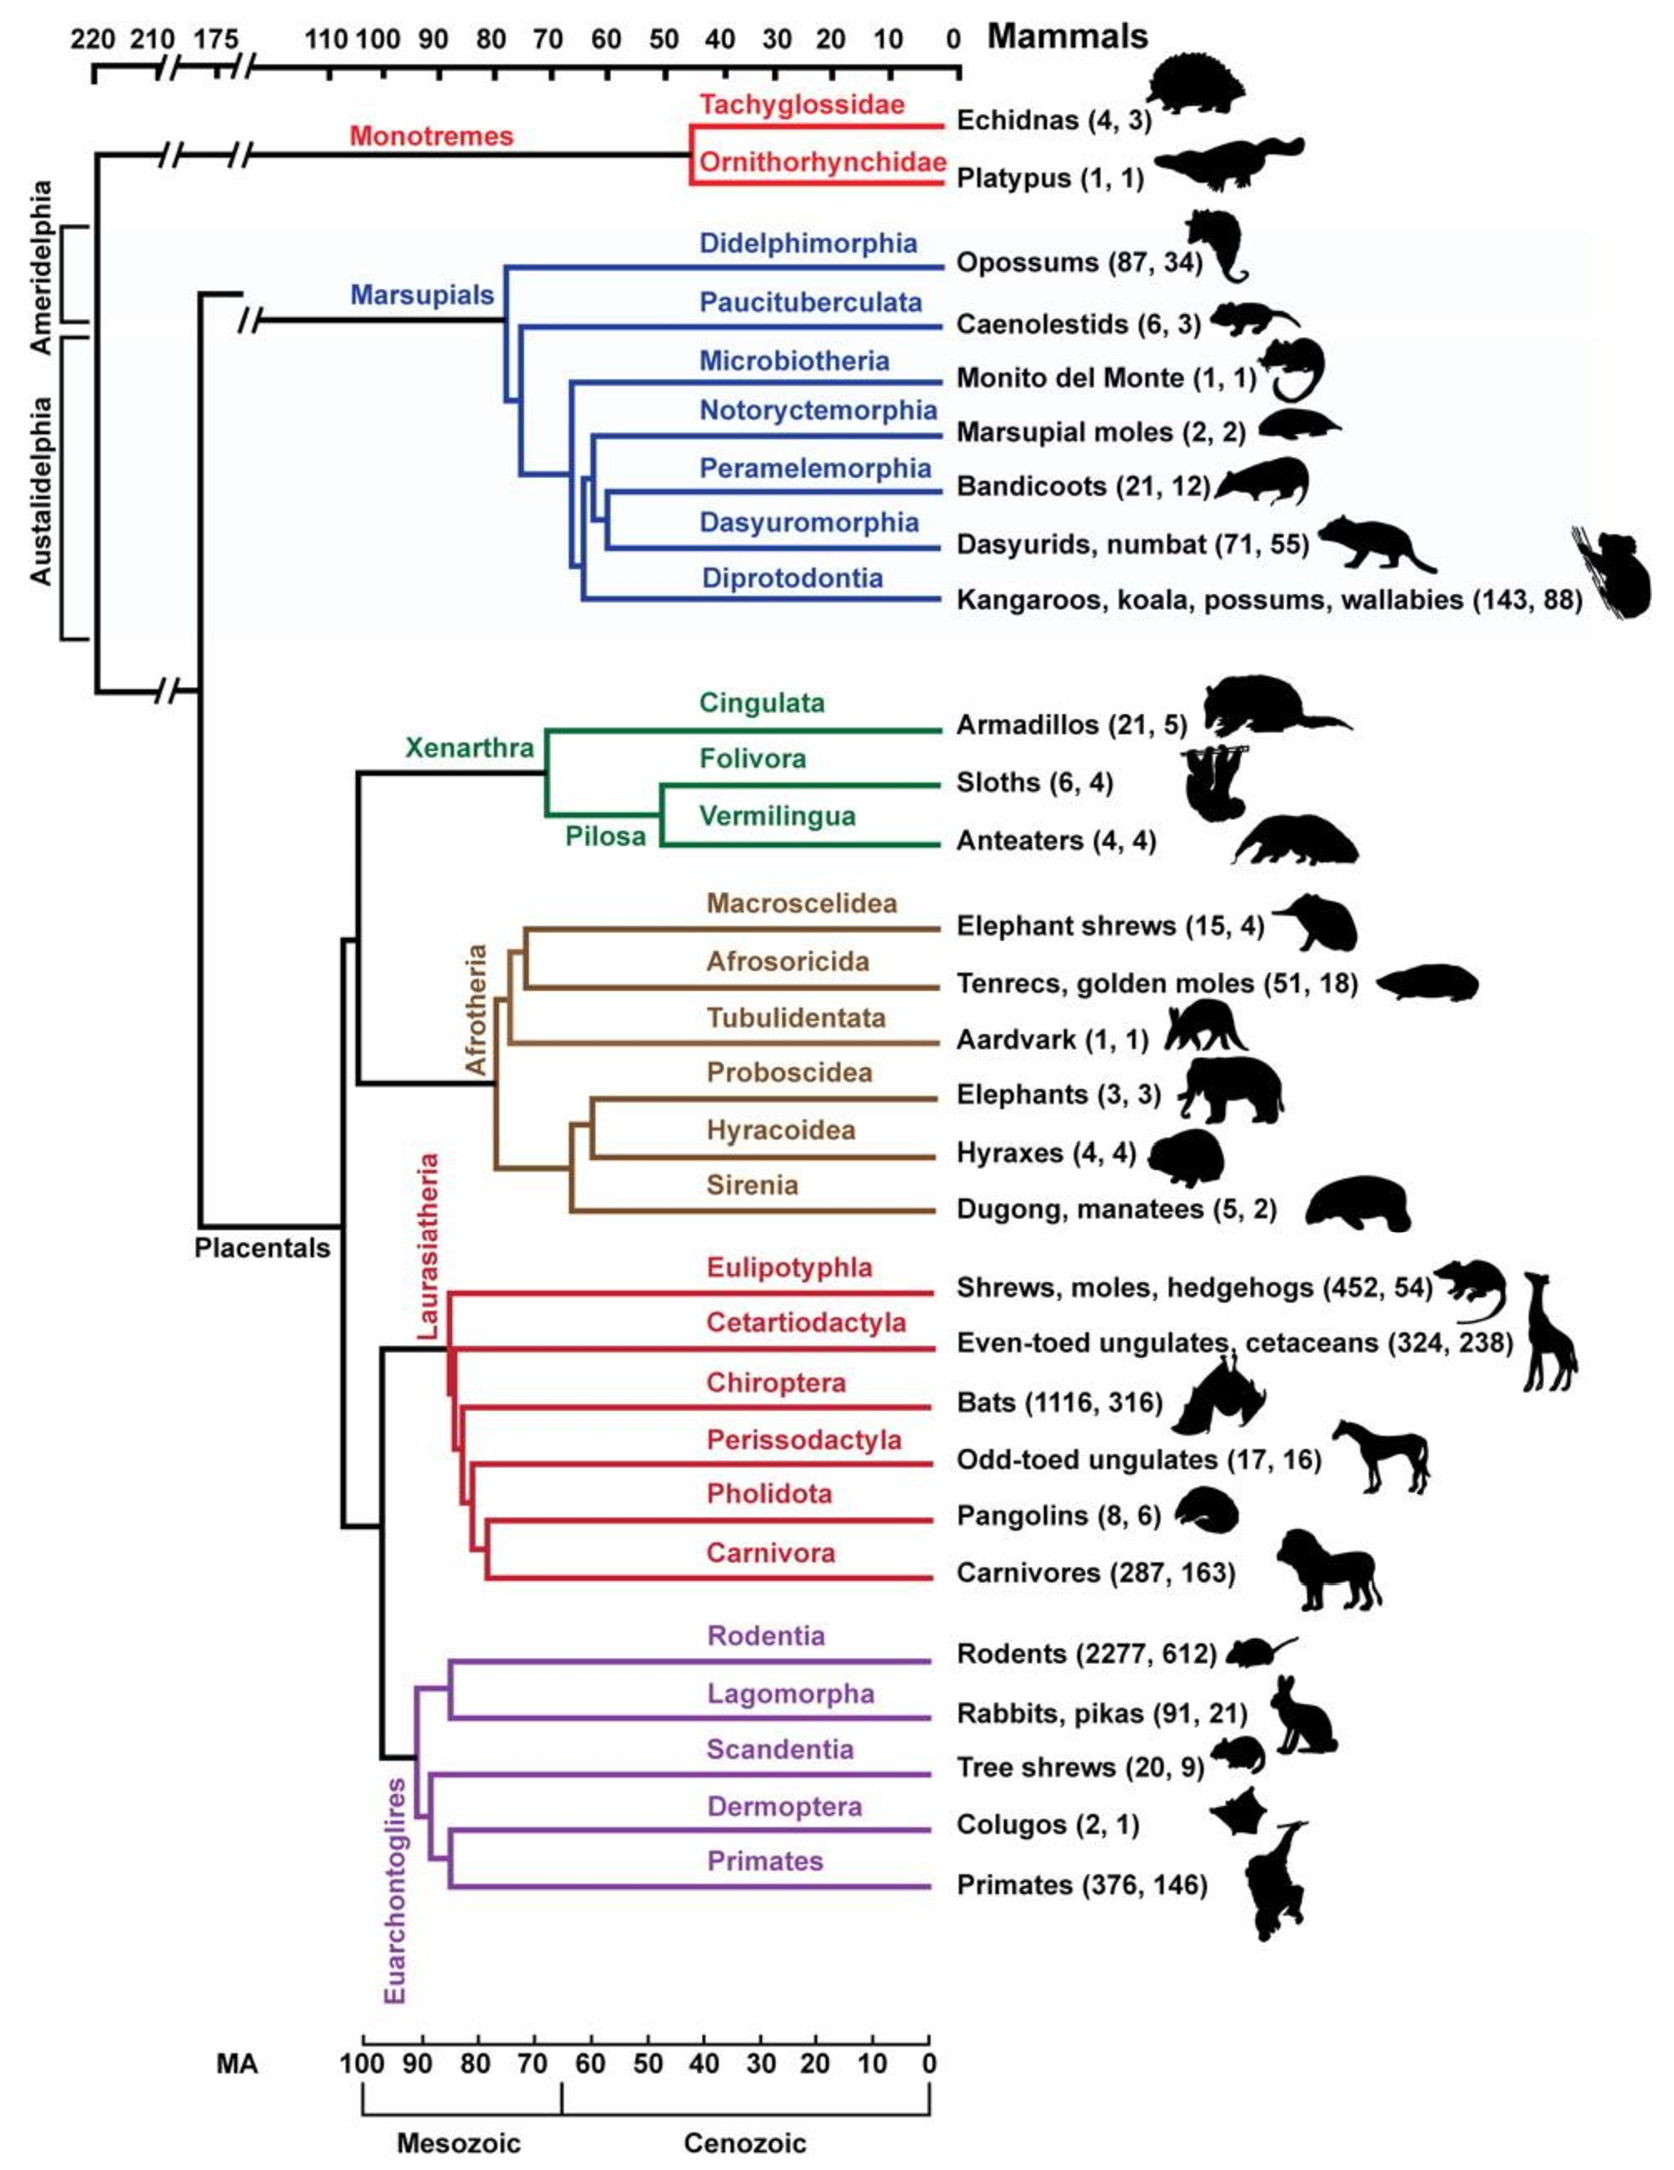
\includegraphics[scale=0.5]{Figs/mammals_10k.pdf}
\caption{A time-resolved consensus phylogeny of the major mammalian
  lineages. Topologies and dates are derived from Hedges and Kumar
  \citeyearpar{Hedges2009}. Each terminal branch represents a
  mammalian family, with the number of species contained in that
  family included as the first number in parentheses (e.g., 2,227
  species of rodents). Figure taken from \citet{Haussler2009}. }
\label{fig_mammals_10k}
\end{figure}

Before the K/T boundary, ancestral mammal and primate species were
small in size, as the ecological niches for larger animals were
occupied by dinosaurs \citep{Martin2008,Smith2010}. Their diets were
likely largely insectivorous, as folivory in extant species is
observed mainly in larger mammals \citep{Smith2010} (but see
\citet{Martin2007} for an alternative perspective favoring a
folivorous primate ancestor). After the K/T extinction event, mammals
eventually diversified to occupy a wide range of the ecological roles
left vacant by extinct species, with many lineages undergoing highly
specialized morphological and behavioral adaptations and the range of
mammalign body sizes expanding by four orders of magnitude
\citep{Alroy1998}. 

The issue of body size is important because... 

Immune system of mammals...

Genome evolution: 2R, transposable elements, genome shuffling...



  \label{evolution_intro}
  \draft{Write a quick summary of the genome evolution of vertebrates
    and mammals. Mention 2R duplication, genome size growth,
    transposable elements.}

  \draft{Introduce the concept of adaptation (molecular
    vs. morphological / ecological), the varied behavioral
    characteristics of modern day mammals (focusing on mammalian
    superorders and great apes, as expanded in mammals and gorilla
    chapters), and the impact of population structure / population
    size on the efficacy of natural selection.}

  \draft{Talk about the evolution of immunity w.r.t. adaptation}


\section{Models of sequence evolution}
\label{codon_intro}

The evolutionary analysis of DNA sequences is a cornerstone of
comparative genomics. As the hereditary material of all free-living
organisms, DNA represents a record of the history of life on
earth. When an individual gives rise to offspring, some segments of
DNA are replicated and passed on to all its descendants; importantly,
this replication process is imperfect, and the resulting
errors---called mutations---are passed on to successive
generations. In addition to being a major source of the variation
between individuals invoked by Darwin's theory of natural selection
\citep{TODO}, mutations in DNA leave a molecular record of
evolutionary relationships and of the passage of time. The gradual
accumulation of mutations in DNA can be modeled using phylogenetic 

The earliest observations that DNA 
were made using the sequences of proteins, which are cellular
molecules comprised of amino acid units whose arrangement is encoded
in stretches of DNA called genes. Zuckerkandl and Pauling, who were
analyzing the amino acid sequences of hemoglobin genes from various
species, noted in 1962 that the number of changes between sequences
corresponded well with the evolutionary distance between species based
on fossil evidence; this led them to hypothesize that evolution at a
molecular level may occur largely at a constant rate
\citep{Zuckerkandl1962,Morgan1998}. Zuckerkandl and Pauling continued
to explore the implications and applications of this notion,
eventually coined as the ``molecular evolutionary clock'' hypothesis,
using hemoglobin and cytochrome C sequences, for example, to estimate
the date of human-gorilla divergence (at 11 million years) and to
infer ancestral protein sequences \citep{Zuckerkandl1965}.

Since those pioneering studies, a wide variety of evolutionary models
have been developed to describe 

  \draft{Introduce the idea of modeling protein evolution as a markov
    process acting on codon sequences: the incorporation of
    mechanistic parameters for Ts:Tv bias (kappa), dN/dS ratio
    (omega), or empirical models a la . Talk about heterogeneity
    the idea that real data may strongly violate certain models.}

\section{Detecting purifying and positive selection in proteins}
\label{pos-sel_intro}

  \draft{Briefly run through the history of detecting purifying /
    positive selection in genes and sites. Mention history of PAML
    models, alternative approaches, and fully describe SLR's
    approach.}

  \draft{SLR implements a method specifically designed for sitewise
    estimates which has been shown in sim- ulations to perform as well
    as or better than PAML’s sitewise random sites models (Massingham
    and Goldman, 2005). SLR models codon evolution as a
    continuous-time Markov process where substitutions at one site are
    independent of substitutions at all other sites. No assumptions
    are made regarding the distribution of ω ratios within the
    alignment. The value of ω is considered to be an independent
    parame- ter at each site: after first optimizing shared parameters
    using the whole alignment, SLR uses the shared parameters and the
    data at each alignment site to calculate a sitewise statistic for
    non-neutral evolution.  This statistic is based on a
    likelihood-ratio test where the null model is neutral evolution (ω
    = 1) and the alternative model is either purifying or positive
    selection (ω < 1 or ω > 1, respectively). The raw statistic
    measures the strength of evidence for non-neutral evolution at
    each site; following Massingham and Goldman (2005) we use a signed
    version of the SLR statistic (created by negating the statistic
    for sites with ω < 1) as the test statistic for positive
    selection.}


\section{Outline of the thesis}

In this thesis, I describe... three studies concerning the use of
phylogenetic codon models to identify

